\documentclass[10pt]{report}
\usepackage[utf8]{inputenc}
\usepackage[italian]{babel}
\usepackage{multicol}
\usepackage[bookmarks]{hyperref}
\usepackage[a4paper, total={18cm, 25cm}]{geometry}
\usepackage{graphicx}
\usepackage{xcolor}
\usepackage{textcomp}
\graphicspath{ {./img/} }
\usepackage{listings}
\usepackage{makecell}
\lstdefinestyle{customasm}{
  belowcaptionskip=1\baselineskip,
  frame=line,
  xleftmargin=\parindent,
  language=[x86masm]Assembler,
  basicstyle=\ttfamily,
  commentstyle=\itshape\color{purple!40!black},
}
\lstset{escapechar=@,style=customasm}
\lstnewenvironment{C}
  {\lstset{language=C++,frame=none}}
  {}
\begin{document}
\title{Computational Mathematics for Learning and Data Analysis}
\author{Federico Matteoni}
\date{A.A. 2021/22}
\renewcommand*\contentsname{Index}

\maketitle
\begin{multicols}{2}
\tableofcontents
\end{multicols}
\pagebreak
\section{Introduction}
Exam: project (groups of 2) + oral exam.\\
This course's goals is to make sense of the huge amounts of data, take something big and unwieldy and produce something small that can be used, a \textbf{mathematical model}.\\
The mathematical model should be accurate, computationally inexpensive and general, but generally is not possible to have all three. General models are convenient (work once, apply many), they are parametric so we need to learn the right values of the parameters. Fitting is finding the model that better represents the phenomenon given a family of possible models (usually, infinitely many). Is an optimization model and usually is the computational bottleneck.\\
ML is better than fitting because fitting reduces the training error, the empirical risk, but ML reduces the test error, so the generalization error.\\
Solve general problem $min_{x\in S}f(x)$, with Poloni solve $min_{x\in R^n}||Ax - b||_2$ which is easier and can be solved exactly.
\paragraph{Quick recap of linear algebra}
\begin{list}{}{}
	\item \textbf{Matrix - Vector multiplication}, with $A\in R^{4\times 3}, c\in R^3, b\in R^4$
	$$\left[\begin{array}{c c c}
		A_{11} & A_{12} & A_{13}\\
		\vdots & \vdots & \vdots\\
		A_{41} & A_{42} & A_{43}
	\end{array}\right]\cdot \left[\begin{array}{c}
		c_1\\c_2\\c_3
	\end{array}\right] = \left[\begin{array}{c}
		b_1\\b_2\\b_3\\b_4
	\end{array}\right]\:\:\:\:\:\:\begin{array}{l}
		b_i = \sum_{j=1}^4 A_{ij}c_j\\
		A_{11}c_1 + A_{12}c_2 + A_{13}c_3 = b_1
	\end{array}$$
	or linear combination of the columns
	$$\left[\begin{array}{c}
	A_{11}\\A_{21}\\A_{31}\\A_{41}
	\end{array}\right]c_1 + \left[\begin{array}{c}
	A_{12}\\A_{22}\\A_{32}\\A_{42}
	\end{array}\right]c_2 + \left[\begin{array}{c}
	A_{13}\\A_{23}\\A_{33}\\A_{43}
	\end{array}\right]c_3 + \left[\begin{array}{c}
	A_{14}\\A_{24}\\A_{34}\\A_{44}
	\end{array}\right]c_4 = \left[\begin{array}{c}
	b_1\\b_2\\b_3\\b_4
	\end{array}\right]$$
	with $c_1, c_2, c_3$ and $c_4$ called coordinates.
	\item \textbf{Basis}: tuple of vectors $v_1, v_2, \ldots, v_n\:|\:$ you can write all vectors $b$ in a certain space as a linear combination $v_1\alpha_1 + v_2\alpha_2 + \ldots + v_n\alpha_n$ with \textbf{unique} $a_1,\ldots,a_n$. The canonical basis is 
	$$c_1 = \left[\begin{array}{c}
	1\\0\\0\\0
	\end{array}\right]\:\:\:c_2 = \left[\begin{array}{c}
	0\\1\\0\\0
	\end{array}\right]\:\:\:c_3 = \left[\begin{array}{c}
	0\\0\\1\\0
	\end{array}\right]\:\:\:c_4 = \left[\begin{array}{c}
	0\\0\\0\\1
	\end{array}\right]$$
	and, for example $$\left[\begin{array}{c}
	3\\5\\7\\9
	\end{array}\right] = \left[\begin{array}{c}
	1\\0\\0\\0
	\end{array}\right]\cdot 3 + \left[\begin{array}{c}
	0\\1\\0\\0
	\end{array}\right]\cdot 5 + \left[\begin{array}{c}
	0\\0\\1\\0
	\end{array}\right]\cdot 7 + \left[\begin{array}{c}
	0\\0\\0\\1
	\end{array}\right]\cdot 9$$
	\item \textbf{Image} $Im A$ = set of vectors $b$ that we can reach with $A$
	\item \textbf{Kernel} $Ker A$ = set of vectors $x\:|\: Ax = 0$ ($x = 0$ is certainly one, there may be others)
	\item \textbf{Invertible} $A$ if this problem has exactly one solution.\\
	$\forall\:b\in R^m$, $A$ must be square and the columns of $A$ are a basis of $R^m \Rightarrow x=A^{-1}b$ where $A^{-1}$ is another square matrix$\:|\: A\cdot A^{-1} = A^{-1}\cdot A = I$ identity matrix (1 on the diagonal, 0 otherwise)\\
	Implementation detail: \texttt{inv(A) * b} is not the best choice. Better: in Python \texttt{scipy.linalg.solv(A, b)} or, in Matlab, \texttt{A \ b}.
	\item \textbf{Cost}, with $A\in R^{m\times n}, B\in R^{n\times p}, C\in R^{m\times p}$ (vectors $\Leftrightarrow n\times 1$ matrices), then the cost of multiplication is $mp(2n-1)$ floating point ops (\textit{flops}), or $O(mnp)$.\\
	In particular, $A, B$ squared $\Rightarrow AB$ costs $O(m^3)$. With $A, v$ vector $\Rightarrow$ $Av$ costs $O(m^2)$. Faster alternatives are not worth it usually. And remember that $AB \neq BA$ generally, and also that $CA = CB \not\Rightarrow A = B$ with $C$ matrix.\\
	If there's $M\:|\: MC = I$, then $A = (MC)A = (MC)B = B$ (multiplying \textit{on the left} by $M$ on both sides)
\end{list}
\paragraph{} Why a real valued function? Strong assumption, given $x'$ and $x''$, I can always tell which one I like best (\textbf{total order} of R). Often more than one objective function, with contrasting and/or incomparable units (ex: loss function vs regularity in ML).\\
But $R^k$ with $k > 1$ has no total order $\Rightarrow$ no \textit{best} solution, only non-dominated ones.\\
Two practical solutions: maximize return with budget on maximum risk or maximize...\\
Even with a single objective function optimization is hard, impossible if $f$ has no minimum in $X$ (so, the problem $P$ is unbounded below. Hardly ever happens in ML, because loss and regularization are $\geq 0$\\
Also impossible if $f > -\infty$ but $\not\exists x$, for example in $f(x) = e^x$. However plenty of $\epsilon$-approximate solutions ($\epsilon$-optima). On PC $x\in R$ is in fact $x\in Q$ with up to 16 digits precision, so approximation errors are unavoidable anyway. Exact algebraic computation is possible but usually slow, and ML is going the opposite way (less precision: floats, half, small integer weights\ldots).\\
Anyway finding the exact $x_*$ is impossible in general.
\paragraph{Norms}
\paragraph{Eigenvalues and eigenvectors}
\paragraph{Semidefinite}
\paragraph{Recall theorem} $\lambda_{min}(x^T x) \leq x^T Q x \leq \lambda_{max}(x^T x)$ for all symmetric $Q$ so $\lambda_{min} \leq \frac{x^T Q x}{x^T x} \leq \lambda_{max}$\\
Slightly different form $\lambda_{min} \leq z^T Q z \leq \lambda_{max}$ for all vectors $z$ with $||z|| = 1$. Equivalent to the other form with $x = \alpha z$, for $\alpha = ||x||$ and a vector $z$ with $||z|| = 1$
$$ \frac{x^T Q x}{x^T x} = \frac{(\not\alpha z)^T Q (\not\alpha z)}{\alpha^2}$$
\paragraph{Generalization for complex matrices} $||x||^2 = |x_1|^2 + \ldots + |x_n|^2$, $x^T \longrightarrow \overline{x^T} = x^*$. For orthogonal matrices $U^*U=I \Rightarrow U$ is unitary. For symmetry $Q^* = Q \Rightarrow Q$ is Hermitian.
% fine recap lin alg
\paragraph{Singular Value Decomposition} Each $A\in R^{n\times n}$ can be decomposed as $A = U\Sigma V^T$ with $U, V$ orthogonal and $\Sigma$ diagonal with $\sigma_i$ on the diagonal with $\sigma_1 \geq \ldots \geq \sigma_n \geq 0$.\\
The first notable difference is it exists for every square matrix. The second difference is $V^T$ which is not the inverse of $U$.\\
Another notation is $[u_1|u_2|\ldots|u_m]\left[\begin{array}{c c c c}
\sigma_1\\ & \sigma_2\\ & & \ddots\\ & & & \sigma_m
\end{array} \right]\left[\begin{array}{c}
v_1^T\\v_2^T\\\vdots\\v_m^t
\end{array} \right] = u_1\sigma_1 v_1^T + \ldots + u_m\sigma_m v_m^T$ sum of $m$ rank-1 matrices\\
Geometric idea: there is an orthogonal basis $v_1,\ldots, v_m$ so that $A$ maps $\{v_i\}$ into multiples of another orthogonal basis $A v_i = u_i \sigma_i$\\
$\{\sigma_i\}$: singular values of $A$, defined uniquely for each $A$\\
Rectangular SVD: each $A\in R^{m\times n}$ can be decomposed as $A = U\Sigma V^T$ where $U\in R^{m\times m}$, $V \in R^{n\times n}$ are orthogonal and $\Sigma\in R^{m\times n}$ is diagonal, so $\sigma_{i,j} = 0$ whenever $i\neq j$ again with $\sigma_1 \geq \ldots \geq \sigma_{min(m, n)} \geq 0$\\
So only the first $n$ vectors of $U$ matches with non-zero values in $\Sigma$, all the last $n-m$ columns combine with zeroes.\\
$= u_i\sigma_1 v_1^T + \ldots + u_n \sigma_n v_n^T$ with $u_{n+1},\ldots, u_m$ not used. So we can "chop off" the unused parts and get the same result.\\
$= u_i\sigma_1 v_1^T + \ldots + u_{min(m, n)} \sigma_{min(m, n)} v_{min(m, n)}^T$\\
In Matlab, \texttt{svd(A, 'econ')} costs $max(m,n)\cdot min(m,n)^2$, still cubic but linear in the largest dimension. the full \texttt{[U, S, V] = svd(A)} cannot be linear because one of the outputs will be a huge orthogonal matrix of $max(m,n)\times max(m,n)$, so it will cost more in time and memory.\\\\
The rank of a matrix $A$ is equal to the number of non-zero $\sigma_i$. $\sigma_1\geq \ldots$ so at one point a $\sigma_r > \sigma_{r+1} = \ldots = \sigma_{min(m,n)} = 0$\\
Given $A = U\Sigma V^T$ we can compute $A^T A = (U\Sigma V^T)^T(U\Sigma V^T) = V\Sigma^T U^T U \Sigma VV^T = V\Sigma^T \Sigma V^T$ with $\Sigma^T \Sigma$ diagonal and $V\Sigma^T \Sigma V^T$ is both an eigenvalue decomposition and an SVD. This proved that the eigenvalues of $A^T A$ Are the squares of the singular values of $A$ plus additional zeroes for dimension reasons.
$$||A||_2 = ||U\Sigma V^T||_2 = ||\Sigma V^T||_2 = ||\Sigma||_2 = \Sigma_1$$
$$||A|| = max_{||z|| = 1} ||\Sigma V^T|| = \sqrt{\sigma_1^2 z_1^2 + \ldots + \sigma_n^2 z_n^2} \leq \sigma_1 \sqrt{z_1^2 +\ldots + z_n^2} = \sigma_1||z|| = \sigma_1$$
$$||A||_F = ||U\Sigma U^T|| = \ldots = \Sigma_1$$
\paragraph{Eckart-Young Theorem} Most important property of the SVD decomposition.\\
we are interested in approximating $A$ with matrices of rank $\leq K$, if $K = 1$ this means find two vectors $u, v$ so that $A = u^T v$, with $K=2$ then $A = u_1^T v_1 + u_2^T v_2$. What is "how close": $min_{rank(X) \leq K}||A - X||$. The theorem states that the solution is related to SVD.\\
The optimal solution of $min_{rank(X) \leq X}||A - X||$ is $X = u_1\sigma_1 v_1^T + \ldots + u_k\sigma_k v_k^T$ where $A = u_1\sigma_1 v_1^T + \ldots + u_{min(m,n)}\sigma_{min(m,n)} v_{min(m,n)}^T$ is an SVD, $A = U\Sigma V^T$.

\paragraph{} If $A$ has rank 1, then $A = u\cdot v^T$ and $A_{ij} = u_i\cdot v_j$\\
If $A$ has rank 2, then $A= u_1\cdot v_1^T + u_2\cdot v_2^T$ and $A_{ij} = (u_1)_i\cdot (v_1)_j + (u_2)_i\cdot (v_2)_j$
\paragraph{SVD Approximation} $X_1 = u_i\sigma_1 v_1^T =$ best approximation score of student $i \cdot n \cdot$ best approximation difficulty of exercise $j$\\
As a statistical estimator: suppose my scores are of the form $A_{ij} = u_i v_j + \epsilon_{ij}$ with $\epsilon_{ij}$ being the error in the score for instance gaussian with variance $\lambda$.\\
The rank 1 approx of $(u_1\sigma_1)$, $v_1$ given by SVD is the one that minimizes $\sum (A_{ij} - u_iv_j)^2 = ||A-X_1||_F^2 = \sum \epsilon_{ji}^2$. This is the maximum-likelihood estimation of abilities $(u_1)_i, (v_1)_j$.\\\\
The best rank 2 approximation is $X_2 = u_1\sigma_1 v_1^T + u_2\sigma_2 v_2^T$ which can be viewed as first approximation plus corrections.\\\\
$\sigma_1 >> \sigma_2,\ldots$ then $A$ very close to rank 1.\\
$\sigma_1, \sigma_2 >> \sigma_3,\ldots$ then $A$ very close to rank 2, and so on.
\paragraph{} $X =$ best rank-1 approx of $I$, $X = u_1\sigma_1 v_1^T$, $x_{ij} = (u_1)_j \sigma_1 (v_1^T)_j$\\
Best rank-2 $X_2 = u_1\sigma_1 v_1^T + u_2 \sigma_2 v_2^T$\\
Best rank-3 $X_3 = u_1\sigma_1 v_1^T + u_2 \sigma_2 v_2^T + u_3 \sigma_3 v_3^T$
And so on\ldots\\
The original image was 256$\times$256 $= 2^{16}$ reals. The compressed version, with $k = 25$ we have $256\cdot5\cdot2 + 25$ which is about a factor of 5 less.\\\\
What is $||A - X_k||_F = \sqrt{\sum (a_{ij} - x_{ij})^2} = ||U\Sigma V^T - U[$main diagonal of $\sigma_i$ untile $\sigma_k] V^T|| = ||U([\ldots$ %TODO
$= \sqrt{\sum_{i=k+1}^{min(m,n)} \sigma_i^2}$
%TODO last half of 28/09
\paragraph{Optimization need to be approximate} \begin{list}{}{}
	\item $\{a_i = A(x_i) = f(x_i) - f_*\}$ absolute gap
	\item $\{r_i = R(x_i) = \frac{f(x_i) - f(x)}{|f_*|} ) \frac{A(x_i)}{|f_*|}\}$ relative gap
\end{list}
But in general computing the gap is hard because we don't know $f_*$, which is what we want to estimate. So it's hard to estimate how good a solution is. Could argue that this is the "issue" in optimization: compute an estimate of $f_*$.
\paragraph{Optimization at least possible} The $f$'s spikes can't be arbitrarily narrow, so $f$ cannot change too fast\\
$f$ Lipsichitz continuous (L-c) on $X$: $\exists\: L > 0\:|\:|f(x) - f(y)| \leq L|x - y|\:\:\:\forall x,y\in X$\\
$f$ L-c $\Rightarrow$ doesn't "jump" and one $\epsilon$-optimum can be found with $O(\frac{LD}{\epsilon})$ evaluations by uniformly sampling $X$ with step $\frac{2\epsilon}{L}$\\
Bad news: no algorithm can work in less that $\Omega(\frac{LD}{\epsilon})$, but it's the worst case of $f$ (constant with one spike).\\
Number of steps is inversely proportional to accuracy: just not doable for small $\epsilon$. Dramatically worse with $X\subset R^n$.\\
Also generally $L$ is unknown and not easy to estimate, but algorithms actually require/use it.
\paragraph{Local Optimization} Even if I stumble in $x_*$ how do I recognize it? This is the difficult thing. Simpler to start with a weaker condition: $x_*$ is the local minimum if it solves $min\{f(x)\:|\:f\in X(x_*, \epsilon) = [x_* - \epsilon, x_* + \epsilon]\}$ for some $\epsilon > 0$.\\
Stronger notion: \textbf{strict} local minimum if $f(x_*) < f(y)$\\
$f$ (strictly) unimodal on X if has minimum $x_* \in X$ and it is (strictly) decreasing on the left $[x_-, x_*]$ and (strictly) increasing on the right $[x_*, x_+]$\\
Most functions are not unimodal, but they are if you focus on the attraction basin of $x_*$ and restrict there. Unfortunately it's true for every local optimum, they all look the same.\\
Once in the attraction basin, we can restrict it by evaluating $f$ in two points and excluding a part. %TODO grafico e formula
How to choose the part so that the algorithm go as fast as possible? Each iteration dumps the left or the right part, don't know which $\Rightarrow$ should be equal $\Rightarrow$ select $r \in (\frac{1}{2}, 1), x'_- = x'_- + (1 - r)D, x'_+ = x_- + rD$\\
Faster if $r$ larger $\Rightarrow$ $r = \frac{D}{2} + \epsilon = x'_\pm = x_- + \frac{D}{2} \pm \epsilon$ but next iteration will have two entirely different $x'_-, x'_+$ to evaluate $f$ on.
\paragraph{Optimally choosing the iterates} A generally powerful concept is to optimize the worst-case behavior $\Rightarrow$ shrink the intervals as quickly as possible.\\
Each iteration dumps either $[x_-, x_-']$ or $[x_+', x_+]$, we don't know which so they should be of equal size $\Rightarrow$ select $r\in (\frac{1}{2},1)$ so that $x_-' = x_- + (1-r)D$ and $x_+' = x_- + rD$\\
$r$ larger $\Rightarrow$ faster convergence, so $r = \frac{D}{2} + \epsilon \Leftrightarrow x_\pm' = x_- + \frac{D}{2}\pm\epsilon$ but next iteration will have two entirely different $x_-', x_+'$ to evaluate $f$ on.\\\\
So we actually want to minimize function evaluations by reusing the surviving point. $$r : 1 = (1 - r) : r \Leftrightarrow r\cdot r = 1 - r \Leftrightarrow r = \frac{\sqrt{5} - 1}{2} = 0.618 = \frac{1}{g}$$ with $g$ being the golden ratio, $g = \frac{\sqrt{5} + 1}{2} = 1.618 \Rightarrow g = 1 + r = 1 + \frac{1}{g}$\\
Theorems breed algorithms: \textbf{golden ratio search}\\
%TODO code on p. 40 of 1-first steps.pdf
After $k$ iterations, $x_+^k - x_-^k = Dr^k$ stops when $Dr^k \leq \delta$, so when $k = 2\log\frac{D}{\delta}$: exponentially faster, can work with small $\delta$. Asymptotically optimal if no other information is available. $\delta \neq \epsilon$ but $f$ L-c $\Rightarrow A(x^k) \leq \epsilon$ when $k = 2\log\frac{LD}{\epsilon}$\\
First example of linear convergence $A(x^k) \leq Sr^k \leq \epsilon$ with $r < 1$, as fast as a negative exponential $\Rightarrow k \geq \frac{\log\frac{S}{\epsilon}}{\log\frac{1}{r}}$\\\\
$O(\log(\frac{1}{\epsilon}))$ good, but the constant $\rightarrow\infty$ as $r\rightarrow 1$

\paragraph{Matrix Norms} %TODO
%TODO inizio lezione 24/09
\paragraph{To make it go faster, give it more information} Two points are needed to see in which direction $f$ is decreasing. If we could see this directly we could make it with one point, faster. Look at the linear function that best locally approximates $f$, trusty old first derivative $f'(x)$: slope of the tangent line to the graph of $f$ in $x$\\
First order model of $f$ at $x$: $L_x(y)=f'(x)(y-x) + f(x)$. $L_x(y) = f(y) \forall\:y\in[x-\epsilon, x+\epsilon]$ for some small $\epsilon > 0$. $x_*$ local minimum then $f'(x_*) = 0 =$ root of $f' =$ stationary point. If $f'(x) < $ or $f'(x) > 0$, then $x$ is clearly not a local minimum. Hence, $f'(x) = 0$ for the all local minima (hence in the global minimum as well) but this is true for the local maxima (hence global maximum as well), as well in the plateau and saddle points. To tell them apart, look at the second derivative $f''$.
\begin{center}
	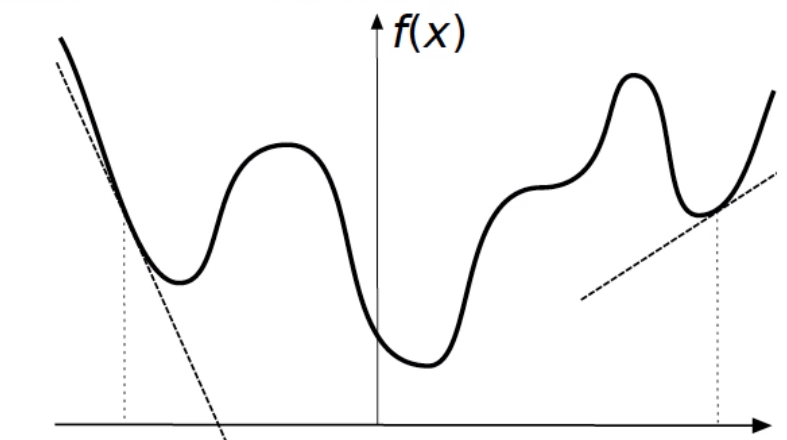
\includegraphics[scale=0.5]{1.png}
\end{center}
In simple cases we get the answer by a closed formula. In $f = bx + c$ linear and $b > 0$ then the minimum is $x_-$ and maximum is $x_+$, viceversa if $b < 0$. For $f = ax^2 + bx + c$ quadratic then if $a > 0$ the minimum is min$\{ x_+, max\{x_*, x_-\}\}$ and the maximum is argmax$\{f(x_-), f(x_+)\}$, and viceversa if $a < 0$.\\
Only polynomial whose root have a closed formula (degree 3 and some degree 4), with basically no hope for most trascendental, trigonometric and mixed equations. We need an algorithm for solving non-linear equations.
\paragraph{Dichotomic Search} $f'$ continuous and the intermediate value theorem gives that $$f'(x_-) < 0 \wedge f'(x_+) > 0 \Rightarrow \exists\:x\in[x_-, x_+]\:|\: f'(x) = 0$$
Theorems breed algorithms $\rightarrow$ \textbf{Dichotomic Search}.\\
%TODO algorithm on page 59 of 1-first steps.pdf
For \texttt{in\_middle\_of(xl, xr)} the obvious choice is \texttt{return (xl + xr)/2;}. We have linear convergence with $\gamma = 0.5 < 0.618 \Rightarrow k = 1.45\log(\frac{LD}{\epsilon}) < 2 \log(\frac{LD}{\epsilon})$\\
The condition $f'(x_-) < -\epsilon, f'(x_+) > \epsilon$ is important. What if is not satisfied? Obvious solution, moving the interval more and more to the right until the derivative is possible. %TODO
The same in reverse of $x_-$ with $\Delta x = -1$. This works in practice for all "reasonable" functions. Works if $f$ coercive ($\lim_{|x| \to \infty} f(x) = \infty$)\\
\begin{list}{}{}
	\item $f' \in C^0 \Leftrightarrow f \in C^1 \Leftrightarrow$ continuously differentiable $\Rightarrow f\in C^0$
	\item $f'' \in C^0 \Leftrightarrow f\in C^2 \Leftrightarrow f' \in C^1 \Rightarrow f' \in C^0 \Rightarrow f \in C^1 \Rightarrow f \in C^0$
	\item $f \in C^1$ globally L-c on $X \Rightarrow |f'(x)| \leq L \forall\: x \in X$
\end{list}
\paragraph{Extreme value theorem} $f \in C^0$ on $X = [x_-, x_+]$ finite $\Rightarrow$ max$\{f(x)\:|\: x\in X\} < \infty$, min$\{f(x)\:|\: x\in X\} > -\infty$\\\\
$f\in C^1$ on $X$ finite $\Rightarrow f$ globally L-c on $X$\\
Best possible case is $f\in C^2$ on finite $X\Rightarrow$ both $f$ and $f'$ globally L-c on $X$
\paragraph{Fastest local optimization} Interpolation, for improving the dichotomic search. Choosing $x$ "right in the middle" is the dumbest possible approach, because we know a lot about $f$: $f(x_-), f(x_+), f'(x_-), f'(x_+)\ldots$. So let's use that, by constructing a model of $f$ based on known information. Much better choosing $x$ close to $x_*$.\\
But remember that the model is an estimate, so never completely trust the model, but regularize, stabilize\ldots in this case, the minimum guaranteed decrease is with $\sigma < 0.5$, and the worst case is linear convergence with $r = 1 - \sigma$, but hopefully is much faster than that when the model is "right".
\paragraph{Measuring algorithms speed} Given the sequences \begin{list}{}{}
	\item $\{x_i\}$
	\item $\{d_i = |x_i - x_*|\}$
	\item $\{f_i = f(x_i)\}$
	\item $\{a_i = A(x_i) = f(x_i) - f_*\}$ absolute gap
	\item $\{r_i = R(x_i) = \frac{f(x_i) - f(x)}{|f_*|} ) \frac{A(x_i)}{|f_*|}\}$ relative gap
\end{list}
We have convergence when $\{a_i\} \rightarrow 0, \{r_i\} \rightarrow 0 \Leftarrow \{d_i\} \rightarrow 0$ (but $\not\Rightarrow)$, but how rapidly? \textbf{Rate of convergence}
$$\lim_{i\to\infty} \left(\frac{f_{i+1} - f_*}{f_i - f_*}\right)^p = \lim_{i\to\infty} \left(\frac{a_{i+1}}{a_i}\right)^p = \lim_{i\to\infty} \left(\frac{r_{i+1}}{r_i}\right)^p = r$$
\begin{list}{}{}
	\item[$p = 1$]\begin{list}{}{}
		\item $r = 1\Rightarrow$ sublinear \begin{list}{}{}
			\item $\frac{1}{i} \Rightarrow k \in O(\frac{1}{\epsilon})$ (bad)
			\item $\frac{1}{i^2} \Rightarrow k \in O(\frac{1}{\sqrt{\epsilon}})$ (a bit better)
			\item $\frac{1}{\sqrt{i}} \Rightarrow k \in O(\frac{1}{\epsilon^2})$ (horrible)
		\end{list}
		\item $r < 1\Rightarrow$ linear, $r_i \rightarrow i \in O(\log(\frac{1}{\epsilon})$, good unless $r = 1$
	\end{list}
	\item[$p \in (1,2)$] $p = 1, r = 0\Rightarrow$ superlinear
	\item[$p = 2$] $r > 0\Rightarrow$ quadratic, best we can reasonably hope for\\
	$\frac{1}{2^{2^i}} \Rightarrow i \in O(\log(\log(\frac{1}{\epsilon})))$, which is basically $O(1)$: the number of correct digits double at each iteration
\end{list}
\paragraph{Improving dichotomic search} Quadratic interpolation has superlinear convergence if started "close enough".\\
$f\in C^3, f'(x_*) = 0 \wedge f''(x_*)\neq 0 \Rightarrow \exists\:\delta > 0\:|\:x_0 \in [x_* - \delta, x_* + \delta] \Rightarrow \{x_i\} \rightarrow x_*$ with $p = \frac{1 + \sqrt{5}}{2}$ exponent of superlinear convergence.\\$x_0$ is the starting point of the algorithm.\\\\
Four conditions $\Rightarrow$ can fit a cubic polynomial and use its minima. Theoretically pays: quadratic convergence ($p = 2$) and seems to work well in practice.
\paragraph{Newton's method} More derivatives, so same information with less points. Construct a second order model $Q_i(x) = Q_{x^i}(x) = f(x^i) + f'(x^i)(x - x^i) + f''(x^i)\frac{(x - x^i)^2}{2}$ and then minimize it.\\\\
$L'_i(x) = L'_{x^i}(x) = f'(x^i) + f''(x^i)(x - x^i) = f'(x)$ and solve $L'_i(x) = 0 \Rightarrow x = x^i - \frac{f'(x^i)}{f''(x^i)}$
\begin{verbatim}
	procedure x = NM(f, x, e)
		while(|f'(x)| > e) do
			x = x - f'(x)/f''(x)
\end{verbatim}
Numerically delicate: what if $f''(x) = 0$? Converges (at all) only if started close enough to $x_*$.\\
If we get within a short enough distance $\delta$, then it will converges extremely fast with $p = 2$. Mathematically, $f\in C^3, f'(x_*) = 0 \wedge f''(x_*)\neq 0\Rightarrow \exists\:\delta>0\:|\:x_0\in[x_*-\delta, x_*+\delta]\Rightarrow \{x_i\} \rightarrow x_*$ with $p = 2$.

\paragraph{Global optimization} Unless strong assumptions are made, we can't say much about global optimization.\\
The obvious one would be unimodal, but not easy to verify/construct. Workable alternative: $f$ convex ($\Rightarrow$ unimodal).
\paragraph{Convexity} $f'$ monotone non decreasing and $f'' \geq 0$. But convexity $\not\Rightarrow C^1$. Some functions are convex and a few operators preserve convexity. Many models are purposely constructed convex $\Rightarrow$  \textbf{Spatial Branch-and-Bound approach}: sift through all $X = [x_-, x_+]$ using clever guide, convex lower approximation \underline{$f$} of nonconvex $f$ on $X$.
\begin{center}
	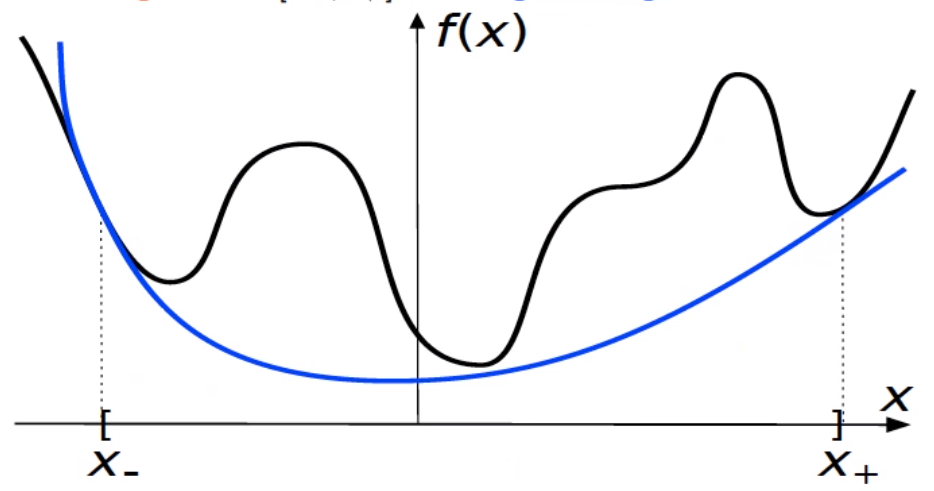
\includegraphics[scale=0.5]{2.png}
\end{center}
"Easily" find local $=$ global minimum $\overline{x}$ giving \underline{$f$}$(\overline{x}) \leq f_* \leq f(\overline{x})$. If gap $f(\overline{x}) - \underline{f}(\overline{x})$ too large, we partition $X$ and iterate. If on some partition $\underline{f}\overline{x}) \geq$ best $f$-value so far, partition killed.\\
In the worst case, exponential complexity because you keep dicing and slicing $X$. But it is exponential in practice too. It depends on how much non-convex $f$ is and how good of a lower approximation $\underline{f}$ is. A cleverer approach is carefully choosing the non-convexities.
%end 1-first steps.pdf
\paragraph{Multivariate} $f$ L-c, no algorithm can work in less than $\Omega((\frac{LD}{\epsilon})^n)$. Curse of dimensionality: not really doable unless $n = 3, 5, 10$ tops. Can make to $O((\frac{LD}{\epsilon})^n)$, with multidimensional grid and small enough step (standard approach to hyperparameter optimization). If $f$ analytic, clever B\&B can give global optimum. If $f$ black-box (typically, no derivatives), many heuristics can give good solutions, probably not optimal.
\subparagraph{Unconstraint global optimization} Local much better: most (but not all) convergence results are dimension indepenteent and not exponential. Doesn't mean that all local algorithms are fast: speed may be low (badly linear), cost of $f$ or derivatives computation increases with $n$ dimension (for large n even $O(n^2)$ may be too much) and some dependency on $n$ may be hidden in $O(\:)$ constraints. Yet, large scale optimization can be done.\\\\
We have a vector space\ldots\\
%TODO 2-uncostrained optimality.pdf, p 20
\paragraph{Tomography} $f:R^n \rightarrow R$ with $x\in R^n$ origin and $d\in R^n$ direction. You can define $\phi_{x,d}(\alpha) = f(x + \alpha d): R \rightarrow R$ tomography of $f$ from $x$ along $d$.\\
$\phi_{x,d}$ can always be pictured, but infinitely many: which $x,d$?\begin{list}{}{}
	\item $||d||$ only changes the scale: $\phi_{x,\beta d}(\alpha) = \phi_{x,d}(\beta \alpha)$ so often convenient to use normalised direction ($||d|| = 1$)
	\item Simplest case: restriction along $i$-th coordinate\\
	$f_x^i(\alpha) = f(x_1,\ldots,x_{i-1},\alpha,x_{i+1},\ldots,x_n) = \phi_{0,u^i}(\alpha)$ with $||u^i|| = 1$
	\item When $x,d$ clear from context, then $\phi(\alpha)$
\end{list}
\paragraph{Simple Functions} \begin{list}{}{}
	\item \textbf{Linear} $f(x) = \langle b,x\rangle + c$\\
	$b \in R^n, c\in R$\\
	Tomography $f(x) = \langle b,x\rangle, x = 0, ||d||=1$: $\phi(\alpha) = \alpha\langle b, d\rangle = \alpha||b||cos(\theta)$\\
	Plotting this gives a line, increasing because "$b$ same direction as $d$", more collinear $\Rightarrow$ steeper. Collinear means steepest line, less collinear means less steap. 90° angle means a flat line. Decreasing if opposite directions.\\
	min $f(x)$ when $\not\exists\:x_*$ if $b \neq 0$ ($\Rightarrow \exists\: d\:|\:\langle b,d\rangle \neq 0$), $\forall\:x$ if $b = 0$
	\item \textbf{Quadratic} %TODO formula
\end{list}
%TODO first half of 5/10
So $B=u_1\sigma_1 v^t$ from SVD of $\overline{A}$ will give me the rank-1 matrix with minimum $||\overline{A}-B||_F^2 = \sum_{i,j}(\overline{A_{i,j}} - B_{i,j})^2$. Suppose now you can only keep a 2D projection of your data. What is the best plane (i.e. minimum sum of squares of errors)? Blue crosses on a plane through the origin = linear combination of tw vectors ($\overline{A}$ = real data, $B$ = plotted data, all cols multiples of the same 2 vectors $\Rightarrow$ rank-2\\
min$||\overline{A}-B|| = $

\end{document}